\def\eg{{\it e.g., \/}}
\def\ie{{\it i.e., \/}}
\def\etal{{\it et al.\/}}
\def\viz{{\it viz.,\/ }}

An attributed flow graph (AFG) $G$, that belongs to a dataset $DS$ of AFGs, is defined as $G = \langle V, E, A, \alpha, w^E, w^V, w^{A,V}, l /rangle$ where:

\begin{enumerate}
\item $V$ is a set of nodes.

\item $E$ is a set of directed edges $(v_a, v_b)$ where $v_a, v_b \in V$.

\item $A$ is the set of all possible attributes.

\item $\alpha$ is a function mapping nodes $v \in V$ to a subset of attributes, \ie $\alpha(v) = \{a_1, ..., a_k\}$,  $a_i \in A$, $1 \leq i \leq k$.

\item $w^E$ is a function assigning a weight $w \in [0,1]$ to each edge $e \in E$ so that $\Sigma_{e \in E_{DS}}w^E(e)$ $ = 1$ where $E_{DS}$ is the set of edges from all AFGs that belong to $DS$, \ie $w^E$ is normalized over $DS$.  

\item $w^V$ is a function assigning a weight $w \in [0,1]$ to each node $v \in V$ so that $\Sigma_{v \in V_{DS}}w^V(v)$ $ = 1$ where $V_{DS}$ is the set of nodes from all AFGs that belong to $DS$, \ie $w^V$ is normalized over $DS$.

\item $w^{A,V}$ is a function assigning a weight $w \in [0,1]$ to each attribute $a$ of each node $v \in V$, $a \in \alpha(v)$, with the constraint that $w^{A,V}(a) \leq w^V(v)$.

\item $l$ is a function assigning a unique integer label $l(v)$ to each node $v \in V$, according to a depth-first traversal of the graph. $l(V)$ denotes the result of applying the labeling function to all nodes in $V$. Given an edge $(v_i, v_j)$, the edge is called a \emph{forward} edge if $l(v_i) < l(v_j)$; otherwise, if $l(v_i) \geq l(v_j)$ the edge is called a \emph{backward} edge or \emph{back-edge}; the node $v_i$ is called the edge's \emph{from-node} and the node $v_j$ is called the edge's \emph{to-node}.   

\item $G$ is a flow graph, \ie for any node $v^*$ it holds that
$\Sigma_{(x, v^*) \in E}w^E((x, v^*))$ $= \Sigma_{(v^*, y) \in E}w^E((v^*, y))$.

\end{enumerate}

A directed graph $g = <V_g, E_g, A_g, \alpha_g, w_g^E, w_g^V, w_g^{A,V}, l_g>$ is a \emph{sub-graph} of $G$, if $V_g$ is a subset of the nodes in $G$, $E_g$ is a subset of the edges in $G$ that exist between nodes in $V_g$, A is a subset of the attributes in $G$, and the functions $\alpha_g, w_g^E, w_g^V, w_g^{A,V}, l_g$ are the corresponding functions in $G$, restricted to the corresponding domains of nodes, edges and attributes in $g$. 

A \emph{pattern} is a graph $P = <V_P, E_P, A, \alpha>$, where $V_P$ is a set of nodes with attributes from $A$ associated to them by $\alpha$, and $E_P$ is a set of directed edges; note that a pattern does not include weights.  A pattern is an abstraction in which the nodes represent sets of attributes that are relevant under a \emph{support criteria}, and the edges represent an ordering for such attribute sets.

An \emph{occurrence} $g$ of a pattern $P$ is a sub-graph of $G$ that ``matches $P$ with a maximum gap size $k_{max}$''; $g$ \emph{matches} $P$ \emph{with a maximum gap size} $k_{max}$ if there is a function $m$ that maps every node $v$ in $P$ to a node in $g$ so that for every edge $(v_i, v_j)$ in $P$, there is a path in $g$ that starts at node $m(v_i)$ and ends at node $m(v_j)$, and that has at most $k_{max}$ nodes between $m(v_i)$ and $m(v_j)$. This definition of an occurrence of a pattern allows a number $k_{max}$ of ``mismatches'' or ``don't-care nodes'' when mapping each edge in the pattern $P$ to a sub-graph in G, and $k_{max}$ can be chosen by a user in order to allow approximate matches in applications where such an approach is useful. A $k-match$ of a pattern $P$ is an occurrence $g_P$ of $P$ that was found by using a gap size of $k_{max}$. As an example, in Figure~\ref{fig:GapExample} we have a pattern on the left and an AFG in which a 0-match, an 1-match and a 2-match of the pattern can be found. 

\begin{figure}[h!]
\centering
%    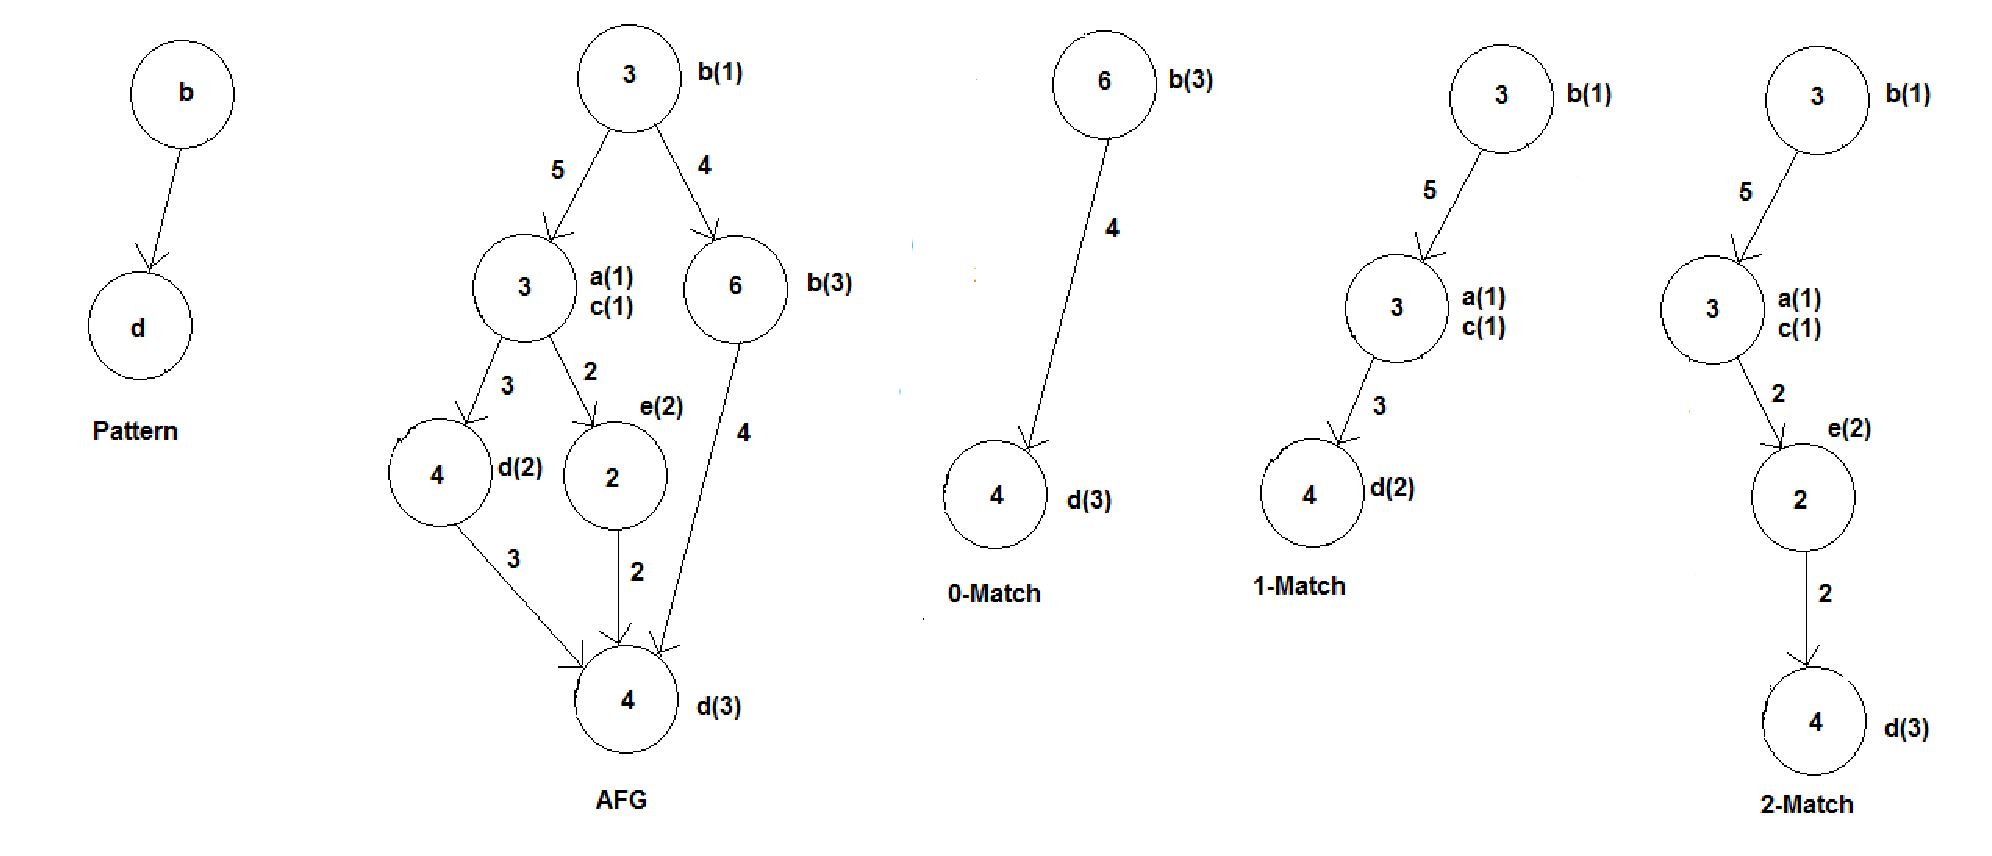
\includegraphics[scale=0.2]{figures/match_example.eps}
      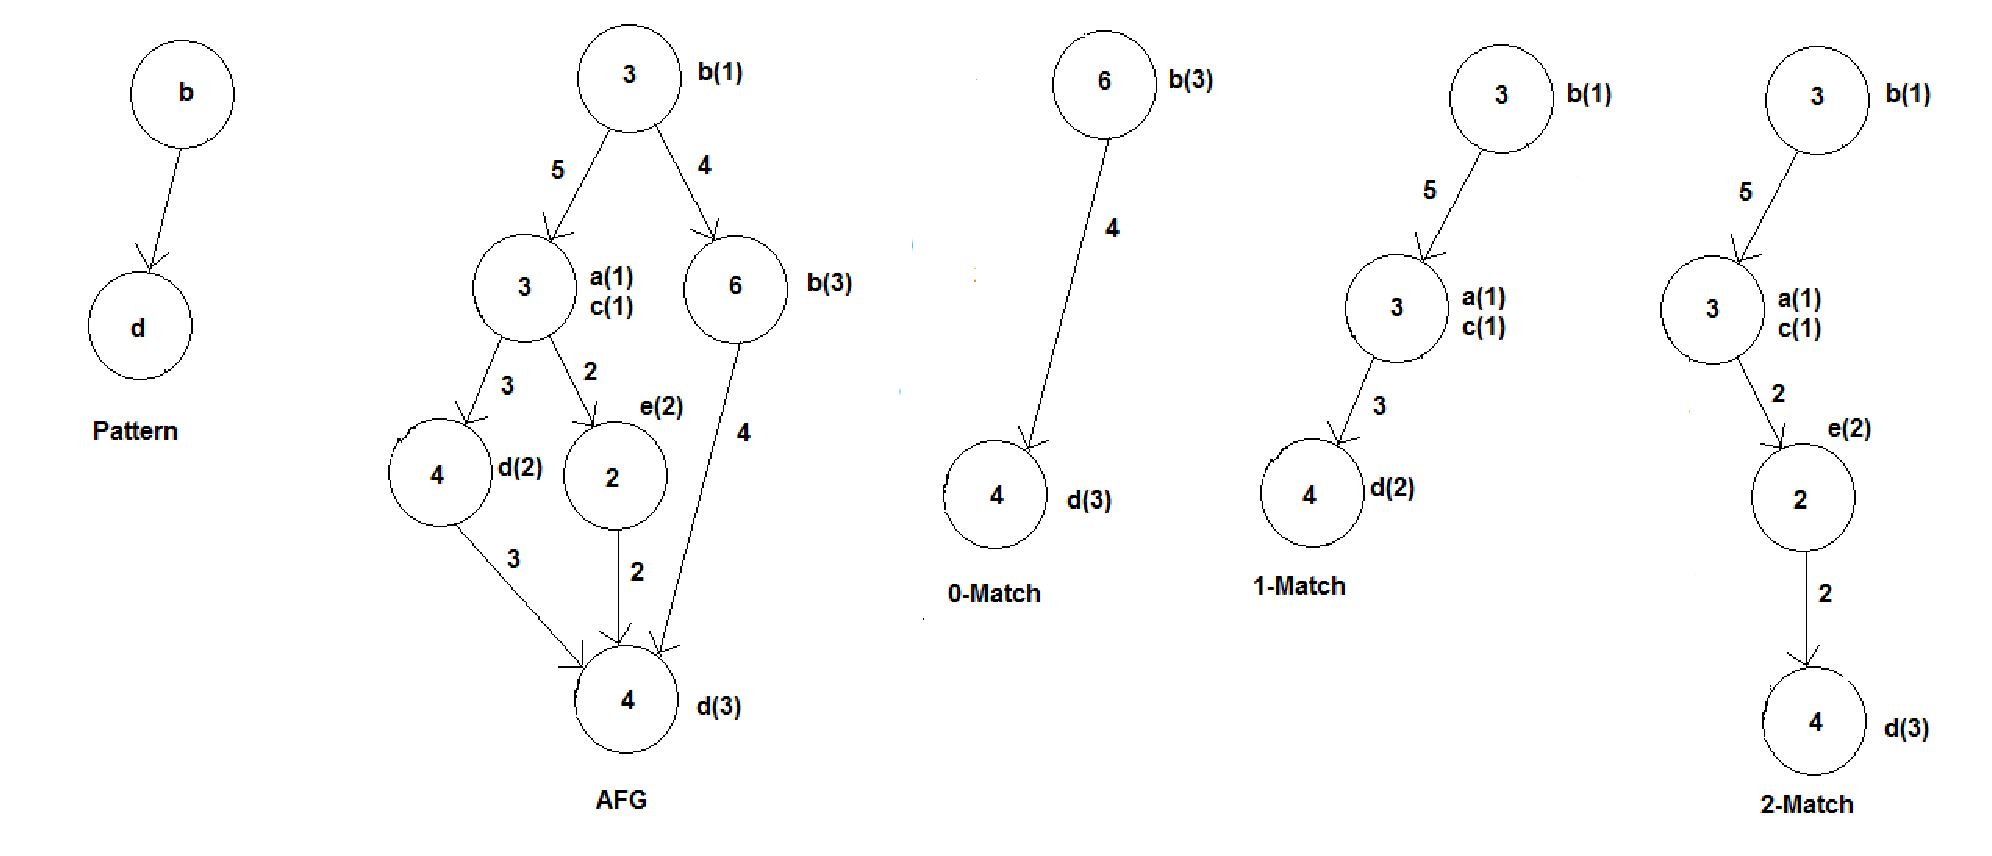
\includegraphics[scale=0.25]{figures/match_example.pdf}
    \caption{Example of k-matches of a pattern.}
    \label{fig:GapExample}  
\end{figure}

Given a dataset $DS$ of AFGs, a \emph{support measure} $F$ that defines the support of patterns $P$ in $DS$, and a threshold value $T$, the problem we address in this paper is to find all patterns $P$ for which $F(P) > T$. We call the patterns for which $F(P) > T$ \emph{heavyweight patterns}, and we call the problem itself {\bf Heavyweight Pattern Mining in Attributed Flow Graphs} (for short, \emph{heavyweight pattern mining}).


